
% ==================================================
%	Theorie
% ==================================================

\section{Theorie}
\subsection{Grundlagen der Röntgenbrechung an einer Grenzschicht}
Ein Röntgenstrahl, welcher durch den elektrischen Feldvektor $\vec{E}(\vec{r})=
\vec{E}_0 \e^{\i\vec{k}\vec{r}}$ beschrieben wird, wird beim Übergang vom Vakuum 
mit Brechungsindex $n_0=1$ in ein Medium mit Brechungsindex 
\begin{equation}
n=1-\delta+\i \beta \label{eq:Brechungsindex} 
\end{equation}
in Abhängigkeit vom Einfallswinkel $\alpha$ zu bestimmten Teilen reflektiert und 
transmittiert. Dabei beschreibt der Realteil des Brechungsindex die neue 
Wellenausbreitung, der Imaginärteil die Abschwächung der Amplitude im 
Medium. Die Schreibweise \eqref{eq:Brechungsindex} mit $\delta > 0$ 
impliziert bereits, dass $\Re(n)<1$, d.h. die Lichtgeschwindigkeit im Medium ist 
größer als im Vakuum.
\begin{itemize}
\item[Aufgabe 1: $\delta>0$] Das Medium wird als eine gleichmäßige Verteilung  
von $N$ harmonischen Oszillatoren der Eingenfrequenzen $\omega_j$ angenommen, sodass 
sich
\begin{equation}
n^2=1+N \frac{e^2}{\epsilon_0 \text{m}} \sum\limits_{j=1}^N \frac{f_j}
{\omega_j^2 - \omega^2-2\i\omega \eta_j}
\end{equation}
ergibt. dabei ist $\omega$ die Frequenz der einfallenden EM-Welle, m die 
Elektronenmasse, $e$ die Elementarladung, $\epsilon_0$ die 
Dielektrizitätskonstante, $\eta_j$ der Dämpfungsfaktor des $j$-ten Elektrons und 
$f_j$ die Stärke der angeregten Schwingung des $j$-ten Elektrons. Für 
Röntgenstrahlung gilt insbesondere $\omega < \omega_j$, sodass für homogene 
Medien die Näherungformel 
\begin{equation}
\delta=\frac{\lambda^2}{2 \uppi} r_e \rho
\end{equation}
für Röntgenstrahlung der Wellenlänge $\lambda$ und Elektronen mit Radius $r_e$ 
und Volumendichte $\rho$ gilt. Folglich ist $\delta$ für Röntgenstrahlung 
positiv und in einer Größenordnung von $10^{-6}$. 
\end{itemize}
Der Übergang in ein Medium mit kleinerem $\Re(n)$ ermöglicht das Phänomen der 
Totalreflexion, sodass bei einem Einfallswinkel $\alpha < \alpha_\text{C}$ mit 
$\cos(\alpha_\text{C})=n$ kein Teil des Strahles transmittiert wird. Der 
Einfallswinkel $\alpha$ wir dabei zwischen Oberfläche und Wellenvektor gemessen. 
Näherungsweise ergibt sich $\alpha_\text{C}=\sqrt{2\delta}$.\\
Sind bei einer Röntgenreflexion $A$, $B$ und $C$ die Amplituden der 
einfallenden, der reflektierten und transmittierten Welle, so gilt für die 
Transmissions- und Reflexionskoeffizienten
\begin{align}
r&=r_s=\frac{B}{A}=\frac{k_\text{i,z}-k_\text{t,z}}{k_\text{i,z}-k_\text{t,z}} \label{eq:r} \\
t&=t_s=\frac{C}{A}= \frac{2 k_\text{i,z}}{k_\text{i,z}+k_\text{t,z}}
\end{align}
wobei $k_\text{i/t,z}$ die $z$-Komponente des Wellenvektors der einfallenden 
bzw. transmittierten Welle ist.
\begin{itemize}
\item[Aufgabe 2 a)] 
Für eine p-Polarisierte EM-Welle ergeben sich 
\begin{align}
r_p&= \frac{n^2 k_\text{i,z}-k_\text{t,z}}{n^2 k_\text{i,z}+k_\text{t,z}} \\
t_p&=\frac{2k_\text{i,z}}{n^2 k_\text{i,z}+k_\text{t,z}}
\end{align}
\item[Aufgabe 2 b)]
Da wie bereits gezeigt $\Re(n)$ nur um $10^{-6}$ von $1$ abweicht, können in 
diesen Formeln die Faktoren $n$ vernachlässigt werden, sodass $r_s=r_p=r$ sowie 
$t_s=t_p=t$ gilt.
\end{itemize}
Die Fresnel-Reflektivität $R_\text{F}=r^2$ kann für Röntgenstrahlung für große 
Einfallswinkel $\alpha_\text{i}$ zu 
\begin{equation}
R_\text{F}\approx \left( \frac{\alpha_\text{C}}{2\alpha_\text{i}} \right)^4 \label{eq:Reflekt4}
\end{equation}
abgeschätzt werden. Dass heißt, die Intensität des Reflexes nimmt mit 
$\alpha_\text{i}^{-4}$ ab, sodass bei der Darstellung eine logarithmische Skala 
zu wählen ist.
\begin{itemize}
\item[Aufgabe 3]
Zu zeigen ist, dass sich \eqref{eq:Reflekt4} aus \eqref{eq:r} ergibt.
\begin{align*}
r=
\end{align*}
\end{itemize}
\subsection{Mehrschichtsysteme}
Nun soll das Problem der Röntgenreflexion auf ein System mit mehreren 
Grenzschichten erweitert werden, speziell wird der im Experiment vorliegende 
Fall einer Probenschicht auf einem Trägermaterial thematisiert.\\
Der Röntgenstrahl fällt aus dem Medium 0 mit $n_0=1$ auf das Medium 
1 (Brechungsindex $n_1$, Schichtdicke $d$) und wird an der Grenzschicht zu $r_1$ 
reflektiert und zu $t_1$ 
transmittiert. Der transmittierte Teilstrahl durchdringt das Medium 1 und trifft 
auf das Trägermaterial (Brechungsindex $2$, Schichtdicke $\to \infty$) und wird 
dort wiederum zu $r_2$ reflektiert und zu $t_2$ transmittiert. Nach Austritt der 
reflektierten Strahlen ergibt sich durch deren Überlagerung eine 
Gesamtreflektivität $R$, welche aufgrund von Interferenzen zwischen den 
reflektierten Strahlen für steigende Einfallswinkel $\alpha$ oszilliert. Sind 
$\alpha_1$ und $\alpha_2$ zwei benachbarte Extremstellen dieser Oszillation, so 
lässt sich die Schichtdicke über
\begin{equation}
d \approx \frac{\lambda}{2(\alpha_2 -\alpha_1)}
\end{equation}
abschätzen.
\begin{itemize}
\item[Aufgabe 4:]
Der Gangunterschied $\Delta l_n$ zwischen zwei Minima muss $\Delta l_n=
(2n+1)/2 \lambda$ betragen, damit die Phasendifferenz $\uppi$ ist. Außerdem 
gilt wegen der Geometrie des Problems, dass $\Delta l_n = 2 d/\sin(\alpha_n)$. 
Aus der Berechnung von $\Delta l_{n+1}- \Delta l_n$ mit $\sin(\alpha)\approx 
\alpha$ (Kleinwinkelnäherung) folgt die angegebene Gleichung für die 
Schichtdicke $d$. Dies ist in Abbildung \ref{fig:Bild} veranschaulicht.
\begin{figure}[h]
\centering
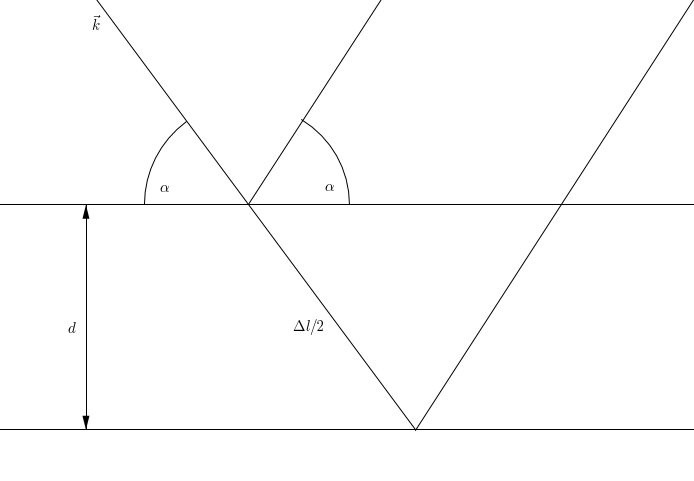
\includegraphics[scale=0.4]{../skript/Bild.png}
\caption{Veranschaulichung der geometrischen Bedingungen zwischen der 
Schichtdicke $d$, dem Einfallswinkel $\alpha$ und dem Gangunterschied $\Delta 
l$.}
\label{fig:Bild}
\end{figure}
\end{itemize}
Die Amplituden $R_j$ und $T_j$ der reflektierten und transmittierten Welle der 
$j$-ten Grenzschicht stehen im Verhältnis
\begin{equation}
X_j:=\frac{R_j}{T_j}=\e^{-2\i k_\text{z,j}z_j} \frac{r_{j,j+1}+X_{j+1}\e^{2\i 
k_\text{z,j+1}z_j}}{1+r_{j,j+1}X_{j+1}\e^{2\i k_{z,j+1}z_j}}
\end{equation}
mit $r_{j,j+1}=\frac{k_{z,j}-k_{z,j+1}}{k_{z,j}+k_{z,j+1}}$ und $k_{z,j}=|
\vec{k}|\sqrt{n_j^2-\cos^2 \alpha_i}$.
\begin{itemize}
\item[Aufgabe 5:]
Eine Darstellung der Gesamtreflektivität $X$ in Abhängigkeit vom Einfallswinkel 
$\alpha$ ist in Abbildung \ref{fig:Mehrschicht} zu sehen.
\begin{figure}[h]
\centering
\includegraphics[scale=1]{../skript/reflektivitaet.pdf}
\caption{Darstellung von $X$ in Abhängigkeit vom Einfallswinkel $\alpha$ für 
eine Rauigkeit von $\sigma=6\AA$ und $n_\text{Substrat}=1-1\times 10^{-6}$.}
\label{fig:Mehrschicht}
\end{figure}
\end{itemize}


\subsection{Die Rauigkeit einer Grenzschicht}
Bisher wurde stets die Annahme gemacht, dass die Grenzschichten eben und ohne 
weitere Struktur sind. Nun wird die Rauigkeit der $j$-ten Genzschicht (bei 
$z=z_j)$ durch eine 
Wahrscheinlichkeitsdichte $P_j$ modelliert, sodass $P_j(z)\,\text{d}z$ die 
Wahscheinlichkeit ist, dass die Grenzschicht in $\text{d}z$ um $z$ liegt. Als 
Maß für die Rauigkeit wird dann
\begin{equation}
\sigma_j^2=\int (z-z_j)^2 P_j(z)\, \text{d}z
\end{equation}
gewählt. Als modifizierter Brechungsindex wird
\begin{equation}
n(z)=\frac{n_j+n_{j+1}}{2}- \frac{n_j-n_{j+1}}{2} \text{erf}\left(\frac{z-z_j}
{\sqrt{2 \sigma^2_j}}  \right)
\end{equation}
benutzt, sodass sich $P_j(z)$ als Gaußfunktion ergibt. Es folgen die neuen 
Fresnel-Koeffizienten
\begin{align}
\tilde{r}_{j,j+1}&=r_{j,j+1} \e^{-2 k_\text{z,j}k_\text{z,j+1}\sigma_j^2} \\
\tilde{t}_{j,j+1}&=t_{j,j+1} \e^{(k_\text{z,k}-k_\text{z,j+1})^2 \sigma_j^2/2}
\end{align}
\begin{itemize}
\item[Aufgabe 6:]
Eine Darstellung des Gesamtreflektivität für ein System mit einer nicht 
verschwindenden Rauigkeit ist in Abbildung \ref{fig:Rauigkeit} zu sehen.
\begin{figure}[h]
\centering
\includegraphics[scale=1]{../skript/reflektivitaet_rau.pdf}
\caption{Darstellung von $X$ in Abhängigkeit vom Einfallswinkel $\alpha$ für 
eine Rauigkeit von $\sigma=6\AA$ und $n_\text{Substrat}=1-1\times 10^{-6}$.}
\label{fig:Rauigkeit}
\end{figure}
\end{itemize}


